\chapter{Ergebnisse} \label{ch:results}

\section{\acs{icd10gm} in der \acs{csv}-Dateien und \acs{db}} \label{sec:dataanalysis}
Die Analyse der Information der \ac{icd10gm} wurde mit Hilfe von \ac{sql}-Befehlen und der Skript Sprache Python unter dem Framework Jupyter-Notebook durchgeführt.

Wie in der Tabelle~\ref{tab:icdfiles} dargestellt wird, jede Kode-Datei enthält mehr als \textsf{15450} Codes, obwohl manche Kodierungen gelöscht werden, nimmt die Menge neuer \ac{icd10gm} ständig zu.

\begin{table}[ht]
	\centering
	\small
	\caption[\acs{icd10gm} in den \acs{csv}-Dateien]{Anzahl an \acs{icd10gm} per Jahr in den \ac{csv}-Dateien}
	\label{tab:icdfiles}
	\begin{tabular}{|l|l|}
		\hline
	\rowcolor{lightgray} Anzahl & Fassung \\ \hline 
		15455 & 2007 \\ \hline
		15498 & 2008 \\ \hline
		15523 & 2009 \\ \hline
		15598 & 2010 \\ \hline
		15633 & 2011 \\ \hline
		15643 & 2012 \\ \hline
		15668 & 2013 \\ \hline
		15688 & 2014 \\ \hline
		15761 & 2015 \\ \hline
		15821 & 2016 \\ \hline
		15930 & 2017 \\ \hline
		16059 & 2018 \\ \hline
		16126 & 2019 \\ \hline
		16131 & 2020 \\ \hline
		16203 & 2021 \\ \hline
		\hline
		\textit{236737} & \textbf{Gesamt} \\ \hline
	\end{tabular}
	\end{table}

Nach dem Durchlauf der \ac{etl} sind insgesamt \textsf{16520} \ac{icd10gm} von 2007 bis 2021 in der \ac{db} eingefügt. In der Abbildung~\ref{fig:icddb} ist die das Verhältnis dieser Kodierungen in Bezug auf die Modifikationen dargestellt. Die meiste Änderungen sind an den Spalten für den Titel der dritte, vierte und fünften Stellen der Codes, weil diese Felder erst im Jahr 2013 entstanden sind \cite{readme13}. Die konkrete Zahl dieser Modifikationen sind in der Tabelle~\ref{tab:icdupd} dargestellt. Ein weiteres Aspekt in Bezug auf der großen Menge der Änderungen ist, dass die Werte verschiedener Felder bei manchen \ac{icd10gm} in früheren Fassungen noch nicht definiert waren, wie in der Tabelle~\ref{tab:icdupd} bei den Fällen der Mortaliätslisten verdeutlicht wird.
 
 \begin{figure}[ht]
 	\centering
 	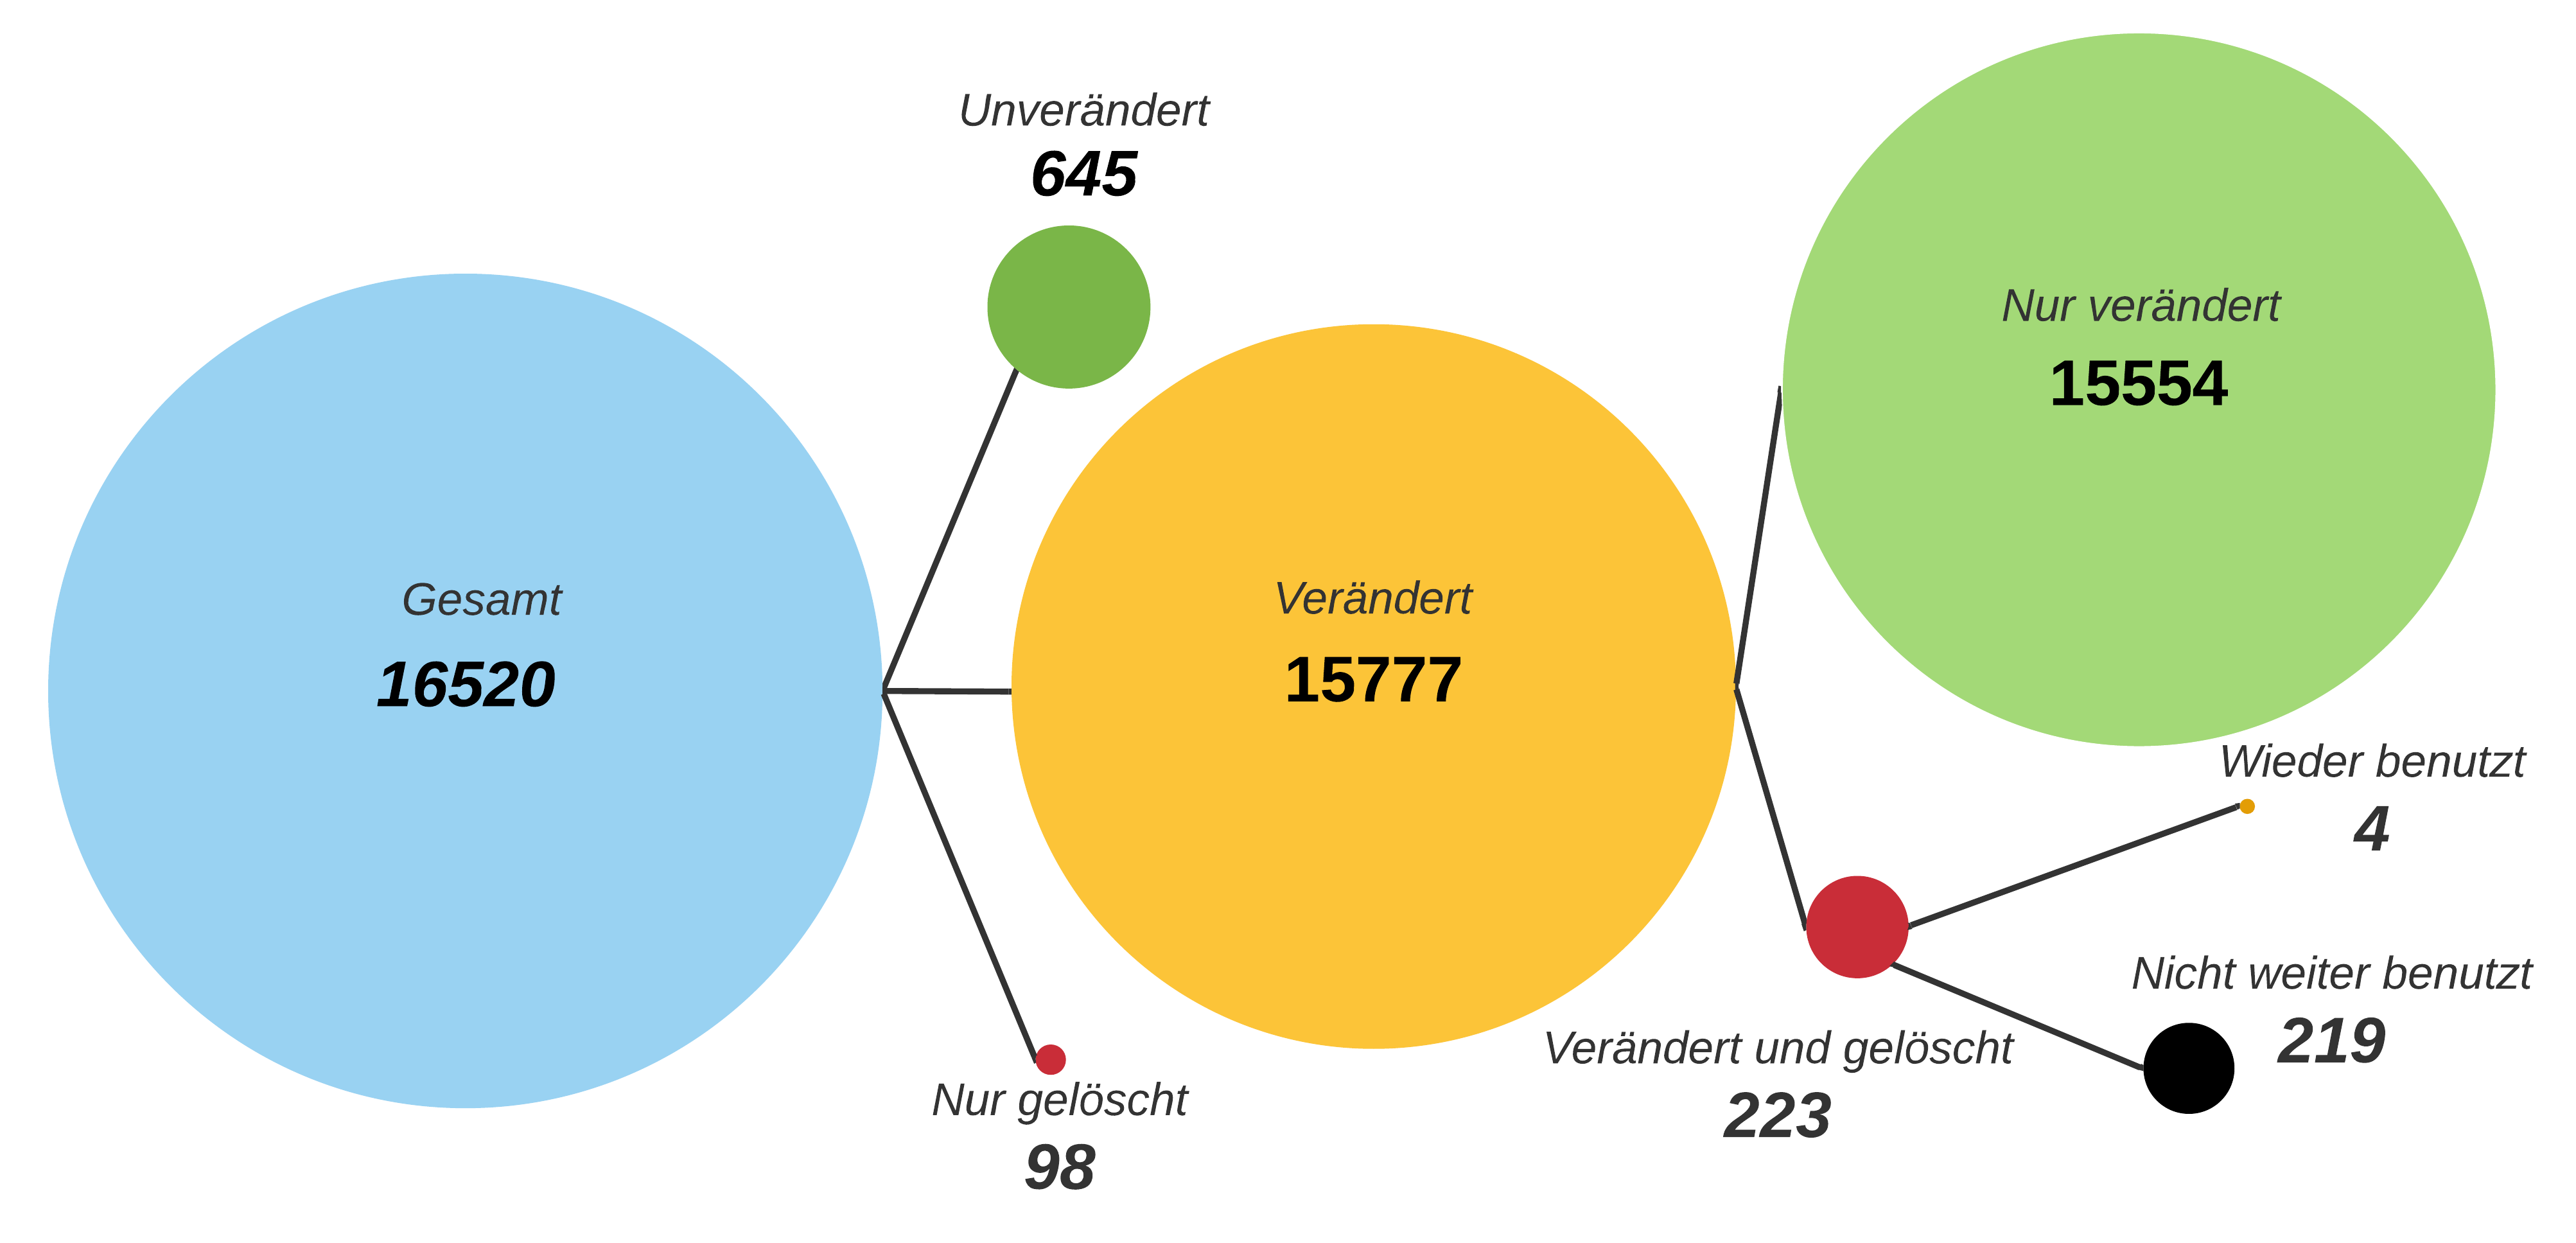
\includegraphics[height=6cm]{figures/icd10gm_quantities}
 	\caption[\acs{icd10gm} in der \acs{db}]{Charakterisierung der \acs{icd10gm} in der \ac{db} in Bezug auf den Modifikationen.}
 	\label{fig:icddb}
 \end{figure}

\section{Neue \acs{icd10gm}} \label{sec:newicd}

Von 2008 bis 2021 sind insgesamt \textsf{966} neuen \ac{icd10gm} entstanden. In der Abbildung~\ref{fig:newicdyear} ist ein interessantes Aspekt davon repräsentiert, nämlich die Anzahl neuer \ac{icd10gm} pro Jahr ist unregelmäßig. Es gib Jahre wie 2017 und 2018 mit mehr als \textsf{120} neue Einträge. Dieses Phänomen passiert am meisten beim Bedarf neuer Subklassifikationen, um die Diagnosen spezifischer zu kodieren und an diverse klinischen Systeme anzupassen. Ein Beispiel dieses Phonemen ist der Code \textsf{U81!} \textsf{Bakterien mit Multiresistenz gegen Antibiotika}, dieser wurde in 2017 entnommen und stattdessen entstand die Kodierung \textsf{U81.-!} \textsf{Gramnegative Erreger mit bestimmten Antibiotikaresistenzen, die besondere therapeutische oder hygienische Maßnahmen erfordern} zusammen mit \textsf{43} weiteren Subklassifikationen von \textsf{U81.0-!} bis \textsf{U81.8!}. Die Ursache davon war eine Umstrukturierung der Bereiche \textsf{U81!}, um diese Codes an die Nomenklatur der \ac{krinko} anzupassen \cite{erreg17}.

Im Jahr 2018 wurden mehr als \textsf{80} neue \ac{icd10gm} in der Bereiche \textsf{M14.-*} \textsf{Arthropathien bei sonstigen anderenorts klassifizierten Krankheiten} eingefügt. Diese Zunahme ist auch in der Abbildung~\ref{fig:newicdcap} widerspiegelt, denn diese Diagnosen sind im Kapitel \textsf{Krankheiten des Muskel-Skelett-Systems und des Bindegewebes} repräsentiert. Die Ursache diese Zunahme war die Insertion einer fünften Stelle an der Kodierung, um die Abbildung im \ac{gdrg}-System zu ermöglichen \cite{musk18}.

%\clearpage

\begin{figure}[ht]
	\centering
	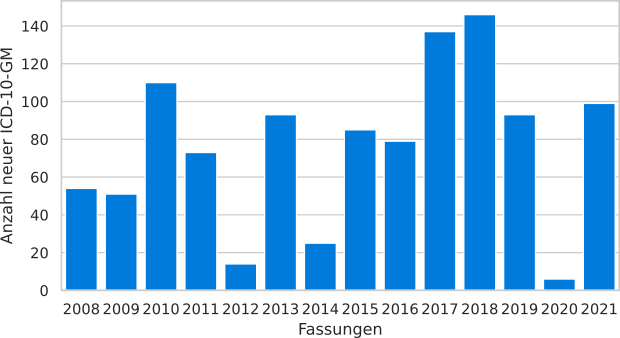
\includegraphics[height=7cm]{figures/newicdyear}
	\caption[Neue \acs{icd10gm} pro Jahr]{Anzahl neuer \acs{icd10gm} zwischen den Jahren 2008 und 2021}
	\label{fig:newicdyear}
\end{figure} 

Ein wichtiger und aktueller Punkt sind die meldepflichtigen Krankheiten in der Laufe der Jahre. Dieses Phonemen ist in der Abbildung~\ref{fig:newicdmeld} dargestellt. Es ist zu erkennen, dass neue meldepflichtigen Codes in den Jahren 2010, 2016 und 2021 definiert wurden (Tabelle~\ref{tab:meldung}). Ursachen davon sind Pandemien und Epidemien wie die Influenza Varianten zwischen 2009 und 2010 \cite{influenza1, influenza2}, die Verbreitung des Dengue Fiebers in Europa als Effekt der Globalisierung mit der steigenden Mobilität \cite{denge1} und Verbreitung der asiatischen Tigermücke \textsl{Aedes (Stegomyia) albopictus} zwischen 2015 und 2016 in der Region als Konsequenz der milden Winter \cite{denge2}, und noch aktuell seit Februar 2020 die Verbreitung des Corona Virus in Europa \cite{corona1} und deren gesundheitlichen Folgen \cite{corona2}. 

Ein interessantes Aspekt der meldepflichtigen Krankheiten in der Tabelle~\ref{tab:meldung} ist die Diagnose \textsf{B17.9} \textsf{Akute Virushepatitis, nicht näher bezeichnet}. Diese Krankheit war unter \textsf{K72.0} \textsf{Akutes und subakutes Leberversagen} zugeordnet, erst in 2010 wurde zur Kenntnis genommen dass, die akute Hepatitis in manche Fälle um eine akute infektiöse Hepatitis handelt. Aus diesem Grund hatte die \ac{who} die Schlüsselnummer \textsf{B17.9} zur Verfügung gestellt \cite{komm10}.

\clearpage

\begin{figure}[ht]
	\centering
	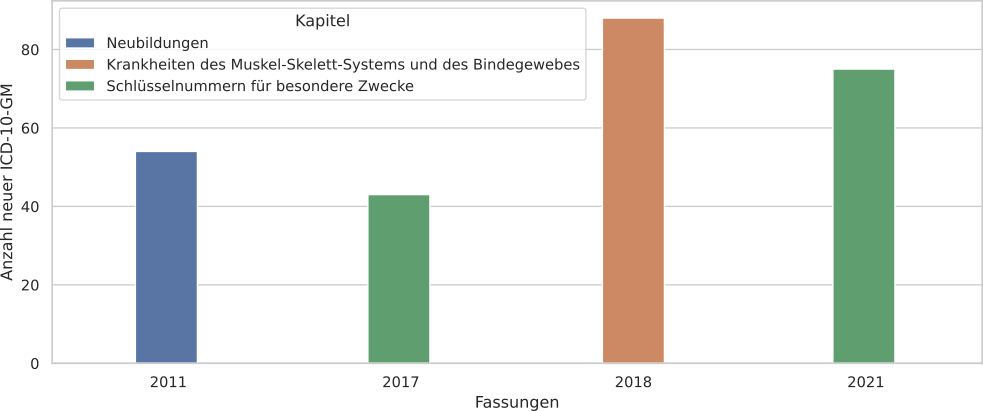
\includegraphics[height=5.7cm]{figures/kaptnrYear}
	\caption[Kapitel mit den meisten eingeführten \acs{icd10gm} (2008 - 2021)]{Kapitel mit den meisten neuen Kodierungen zwischen 2008 und 2021}
	\label{fig:newicdcap}
\end{figure}

%\clearpage
\begin{figure}[ht]
	\centering
	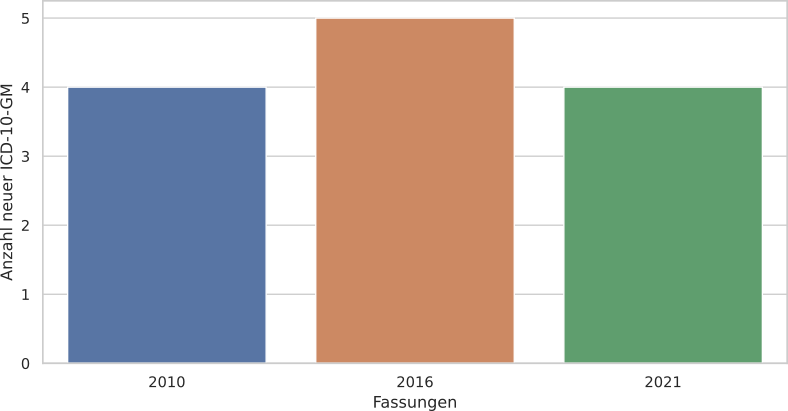
\includegraphics[height=5.7cm]{figures/arztJaYear}
	\caption[Neue meldepflichtige \acs{icd10gm} pro Jahr]{Menge der neuen meldepflichtigen Diagnosen zwischen den Jahren 2008 und 2021}
	\label{fig:newicdmeld}
\end{figure} 

\clearpage
\begin{table}[ht]
	\centering
	\small
	\caption[Meldepflichtige \acs{icd10gm}]{Meldepflichtige Krankheiten}
	\label{tab:meldung}
	\begin{tabular}{|l|l|p{10.5cm}|}
		\hline
		\rowcolor{lightgray} Fassung & \acs{icd10gm} & Titel \\ \hline
		2010 & B17.9 & Akute Virushepatitis, nicht näher bezeichnet \\ \hline
		2010 & U69.2-! & Sekundäre Schlüsselnummern für besondere epidemiologische Zwecke \\ \hline
		2010 & U69.20! & Influenza A/H1N1 Pandemie 2009 [Schweinegrippe] \\ \hline
		2010 & U69.21! & Influenza A/H5N1 Epidemie [Vogelgrippe] \\ \hline
		2016 & A97.- & Dengue \\ \hline
		2016 & A97.0 & Dengue ohne Warnzeichen \\ \hline
		2016 & A97.1 & Dengue mit Warnzeichen \\ \hline
		2016 & A97.2 & Schweres Dengue \\ \hline
		2016 & A97.9 & Dengue, nicht näher bezeichnet \\ \hline
		2021 & U07.1! & COVID-19, Virus nachgewiesen \\ \hline
		2021 & U07.2! & COVID-19, Virus nicht nachgewiesen \\ \hline
		2021 & U10.- & Multisystemisches Entzündungssyndrom in Verbindung mit COVID-19 \\ \hline
		2021 & U10.9 & Multisystemisches Entzündungssyndrom in Verbindung mit COVID-19, nicht näher bezeichnet \\ \hline
	\end{tabular}
\end{table}

\section{Modifizierte \acs{icd10gm}} \label{sec:updicd}

Jedes Jahr werden Änderungen in der Metadaten der \ac{icd10gm} vorgenommen. Solche Modifikationen sind in der Tabelle \ref{tab:icdupd} ausgelistet. In dieser Tabelle ist es zu erkennen, dass die meiste Änderungen in Bezug zur Mortalitätslisten entstanden sind, nämlich \textsf{6949} \ac{icd10gm} bei dem Bezug zur Mortalitätsliste 3 und \textsf{6348} Kodierungen bei dem Bezug zur Mortalitätsliste 1. Die Ursache davon ist, dass die Werte solche Listen bei der meisten Codes im Jahr 2007 nicht definiert waren, und mit dem Wert \textsf{UNDEF} gesetzt. Erst in 2008 wurden diese Felder durch einen spezifischen Wert ersetzt. Die zahlreiche Modifikationen an der Klassentitel entstehen durch Vorschläge zur Weiterentwicklung der Klassifikationen. Ein Beispiel davon ist die Schlüsselnummer \textsf{E10.31} mit dem Titel \textsf{Primär insulinabhängiger Diabetes mellitus [Typ-1-Diabetes] \underline{mit} Augenkomplikationen: Als entgleist bezeichnet}. Dieser Titel wurde zu \textsf{Primär insulinabhängiger Diabetes mellitus [Typ-1-Diabetes] \underline{: Mit } Augenkomplikationen: Als entgleist bezeichnet} in 2009 geändert. Die Änderung wurde in diesem Jahr durchgeführt, da eine fünfte Stelle in der Klassifikationen von \textsf{E10}  bis \textsf{E14} eingefügt wurde \cite{diab09}. Der Titel dieser \ac{icd10gm} wurde nochmal in 2014 zu \textsf{\underline{Diabetes mellitus, Typ 1: Mit Augenkomplikationen: Als entgleist bezeichnet}} ersetzt. In diesem Jahr wurden die Titel von der \ac{who} an die gebräuchliche Terminologie angepasst \cite{komm14}.

%\clearpage

\begin{table}[ht]
	\centering
	\small
	\caption[Änderungen in den Metadaten]{Liste der Metadaten und Anzahl an Änderungen}
	\label{tab:icdupd}
	\begin{tabular}{|l|p{11.5cm}|}
		\hline
		\rowcolor{lightgray} Änderungen & Metadaten \\ \hline
		15578 & Dritte Stelle \\ \hline
		13871 & Vierte Stelle \\ \hline
		6949 & Bezug zur Mortalitätsliste 3 \\ \hline		
		6348 & Bezug zur Mortalitätsliste 1 \\ \hline
		2 & \textbf{Bezug zur Mortalitätsliste 1 (definiert)} \\ \hline
		5061 & Fünfte Stelle \\ \hline
		%1193 & Art des Fehlers bei Geschlechtsbezug \\ \hline
		1111 & Klassentitel \\ \hline
		308 & Untere Altersgrenze \\ \hline
		36 & \textbf{Untere Altersgrenze (relevant)} \\ \hline
		299 & Bezug zur Morbiditätsliste \\ \hline
		11 & \textbf{Bezug zur Morbiditätsliste (definiert)} \\ \hline
		%286 & Alter Fehlertyp \\ \hline
		286 & Obere Altersgrenze \\ \hline
		14 & \textbf{Obere Altersgrenze (relevant)} \\ \hline
		162 & Anwendung der Laborausschlussziffer des \ac{ebmg} \\ \hline
		118 & Art der Vier- und Fünfsteller \\ \hline
		69 & Bezug zur Mortalitätsliste 4 \\ \hline
		68 & Geschlechtsbezug \\ \hline
		64 & Bezug zur Mortalitätsliste 2 \\ \hline
		2 & \textbf{Bezug zur Mortalitätsliste 2 (definiert)} \\ \hline
		44 & Kategorie der Gruppe \\ \hline
		40 & Arzt-Meldepflicht \\ \hline		
		31 & Sehr seltene Krankheit in Mitteleuropa \\ \hline				
		6 & Belegung des Codes \\ \hline
		3 & \S 295 \ac{sgb} V \\ \hline		
		2 & Klassifikationsebene \\ \hline
		
	\end{tabular}
\end{table}

Ein interessantes Aspekt ist, dass \textsf{52} Diagnosen mit Geschlechtsbezug der \textsf{68}, Krankheiten der Brustdrüse sind. Diese \ac{icd10gm} waren frühe auf das weibliche Geschlecht bezogen, jetzt ist der Geschlechtsbezug diese Kodierungen irrelevant. Viele dieser Änderungen wurden in den Jahren 2008 und 2016 vorgenommen. An dieser Stelle können wir nicht erklären, wieso diese Art von Krankheiten nicht immer ohne Geschlechtsbezug waren, denn seit 1930 existieren medizinische Publikationen über Brustdrüse Anomalien bei Männer \cite{bcm}. 

\begin{table}[ht]
	\centering
	\caption[Diphtherie und Poliomyelitis]{\ac{icd10gm} der Bereiche \textsf{A36.-} \textsf{Diphtherie} und \textsf{A80.-} \textsf{Akute Poliomyelitis [Spinale Kinderlähmung]}. \textsf{J} Ja, \textsf{N} Nein.}
	\label{tab:icdeuropa}
	\begin{tabular}{|l|l|p{8cm}|l|l|}
		\hline
		\rowcolor{lightgray} Änderung & \ac{icd10gm} & Titel & Alt & Neue \\ \hline
		2011 & A36.- & Diphtherie & N & J \\ \hline
		2011 & A36.0 & Rachendiphtherie & N & J \\ \hline
		2011 & A36.1 & Nasenrachendiphtherie & N & J \\ \hline
		2011 & A36.2 & Kehlkopfdiphtherie & N & J \\ \hline
		2011 & A36.3 & Hautdiphtherie & N & J \\ \hline
		2011 & A36.8 & Sonstige Diphtherie & N & J \\ \hline
		2011 & A36.9 & Diphtherie, nicht näher bezeichnet & N & J \\ \hline
		2011 & A80.- & Akute Poliomyelitis [Spinale Kinderlähmung] & N & J \\ \hline
		2011 & A80.0 & Akute paralytische Poliomyelitis durch Impfvirus & N & J \\ \hline
		2011 & A80.1 & Akute paralytische Poliomyelitis durch importiertes Wildvirus & N & J \\ \hline
		2011 & A80.2 & Akute paralytische Poliomyelitis durch einheimisches Wildvirus & N & J \\ \hline
		2011 & A80.3 & Sonstige und nicht näher bezeichnete akute paralytische Poliomyelitis & N & J \\ \hline
		2011 & A80.4 & Akute nichtparalytische Poliomyelitis & N & J \\ \hline
		2011 & A80.9 & Akute Poliomyelitis, nicht näher bezeichnet & N & J \\ \hline
	\end{tabular}
\end{table}

In Bezug auf die sehr seltene Krankheiten in Mitteleuropa sind \textsf{20} von den \textsf{31} belegte Schlüsselnummer. Davon gehören \textsf{14} zu den Bereichen \textsf{A36.-} \textsf{Diphtherie} und \textsf{A80.-} \textsf{Akute Poliomyelitis [Spinale Kinderlähmung]}. Diese sind in der Tabelle \ref{tab:icdeuropa} ausgelistet. Die Ursachen der Änderungen sind die erfolgreiche Impfkampagne in Deutschland, sodass die vom \ac{rki} jährlich selten gemeldeten Fällen importiert sind \cite{dippol1}.

\section{Gelöschte \acs{icd10gm}} \label{sec:deletedicd}

In jeder Fassung von 2008 bis 2021 \ac{icd10gm} werden gelöscht. Dieses Verhalten ist in der Abbildung \ref{fig:newdeleteoldicdyear} repräsentiert. Die meiste davon im Jahr 2013. 

\clearpage
\begin{figure}[ht]
	\centering
	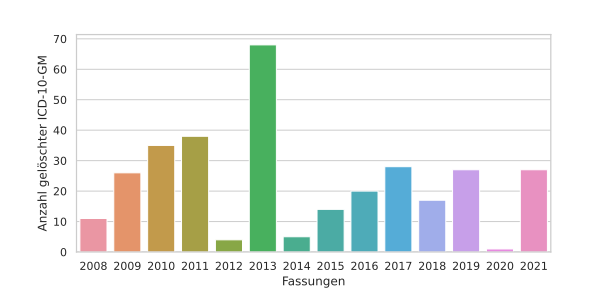
\includegraphics[height=6cm]{figures/neuVersionDelete}
	\caption[Gelöschte \acs{icd10gm} pro Jahr]{Anzahl gelöschten \acs{icd10gm} zwischen den Jahren 2008 und 2021}
	\label{fig:newdeleteoldicdyear}
\end{figure} 

%\clearpage

\begin{figure}[ht]
	\centering
	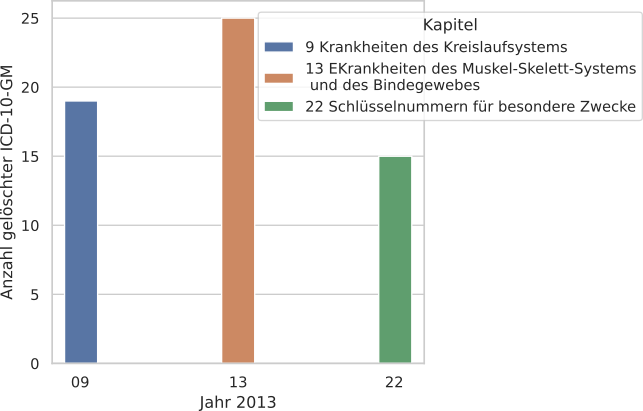
\includegraphics[height=6cm]{figures/kaptnr13}
	\caption{Meist betroffene Kapitel in 2013}
	\label{fig:kap13}
\end{figure}

Die Kapitel, die in diesem Jahr, am meisten getroffen wurden, sind in der Abbildung \ref{fig:kap13} dargestellt. In diesem Jahr wurde eine umfangreiche Umstrukturierung in der Semantik vorgenommen, bei denen bestimmte Kodebereiche im Kapitel \textsf{09} \textsf{Krankheiten des Kreislaufsystems} umfänglich überarbeitet wurden, viele fünfstellige Klassifizierungen wurden von Kapitel \textsf{13} \textsf{Krankheiten des Muskel-Skelett-Systems und des Bindegewebes} entnommen, und im Kapitel \textsf{22} \textsf{Schlüsselnummern für besondere Zwecke} wurden zahlreiche \ac{icd10gm} umgebaut \cite{dele13}.

Die Abbildung \ref{fig:oldicdort} zeigt, dass die meiste Codes, nämlich \textsf{295} der \textsf{327} gelöschten Kodierungen, terminale Schlüsselnummer waren, also \ac{icd10gm} ohne Subkategorien. Davon wurden \textsf{115} erweitert wie in der Sektion \ref{sec:newicd} erläutert wurde. Von der nicht terminale Kodierungen wurden dann \textsf{11} erweitert. Ein Beispiel davon ist \textsf{Z75.2-} \textsf{Wartezeit auf eine Untersuchung oder Behandlung}, diese nicht terminale Kodierung wurde gelöscht und zu der terminalen Code \textsf{Z75.2} mit demselben Titel umgewandelt. Der Rest der \ac{icd10gm} wurden einfach nicht mehr weiter benutzt. 

%\clearpage

\begin{figure}[ht]
	\centering
	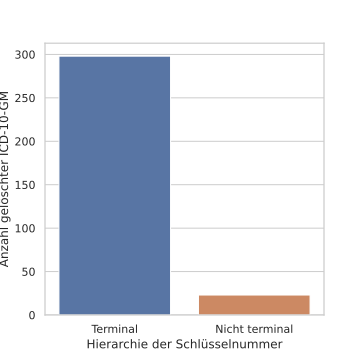
\includegraphics[height=6cm]{figures/ortoldYear}
	\caption{Hierarchie der gelöschte \acs{icd10gm}}
	\label{fig:oldicdort}
\end{figure}

%\newpage

\section{Wiederverwendete \acs{icd10gm}} \label{sec:delinicd}

Die Tabelle \ref{tab:wieder} zeigt die \textsf{4} Schlüsselnummer, die wiederverwendet wurden.

\begin{table}[ht]
	\centering
	\small
	\caption[Wieder benutzte \acs{icd10gm}]{Liste der wieder benutzten \ac{icd10gm}}
	\label{tab:wieder}
	\begin{tabular}{|l|l|l|p{6cm}|}
		\hline
		\rowcolor{lightgray} Gelöscht & Wieder & \ac{icd10gm} & Aktueller Titel \\ \hline
		2013 & 2015 & M21.60 & Erworbener Hohlfuß [Pes cavus] \\ \hline
		2013 & 2015 & M21.6- & Sonstige erworbene Deformitäten des Knöchels und des Fußes \\ \hline
		2014 & 2016 & N90.8 & Sonstige näher bezeichnete nichtentzündliche Krankheiten der Vulva und des Perineums \\ \hline
		2010 & 2019 & K55.8 & Sonstige Gefäßkrankheiten des Darmes \\ \hline

\end{tabular}
\end{table}

Die Schlüsselnummer \textsf{M21.6-} und \textsf{M21.60} wurden in 2013 entnommen, da im Kodebereich \textsf{M20-M25} zahlreiche Schlüssel zu keine sinnvolle Kombinationen führten \cite{dele13}. Andererseits in 2015 wurde die Kategorie \textsf{M21.6} mit den genannten Schlüsselnummer wieder aufgenommen, um eine bessere Spezifikation der Diagnosen in dem \ac{gdrg}-System \cite{komm15}. 

Die \ac{icd10gm} \textsf{N90.8} wurde in 2014 entnommen und stattdessen wurde \textsf{N90.8-} \textsf{Sonstige näher bezeichnete nichtentzündliche Krankheiten der Vulva und des Perineums} mit weiteren Subklassifikationen zur spezifischen Kodierung eingeführt \cite{komm14}. Zwei Jahre später in 2016 wurde der Code \textsf{N90.8-} und deren Unterkategorien wieder entnommen und zu anderem Kapitel mit neuen Codes verlagert, und die Schlüsselnummer \textsf{N90.8} wurde wieder eingeführt \cite{komm16}.

Die Kodierungsschlüssel \textsf{K55.8} wurde in 2010 gelöscht und die Kodierung \textsf{K55.8-} \textsf{Sonstige Gefäßkrankheiten des Darmes} mit weiteren Stellen eingeführt, um einige Diagnosen des Dünndarms bessern abgrenzen zu können \cite{komm10}. In 2019 wurde die \ac{icd10gm} \textsf{K55.3-}   \textsf{Angiodysplasie des Dünndarmes} mit weiteren fünfstelligen Codes eingeführt und die, in 2010, eingeführte Klassifikationen wurden auf dem neuen Kodeberich verlagert, sodass die Kodierungen von 2010 obsolet wurden, und \textsf{K55.8} wieder benutzt wurde \cite{komm19}.

\section{Strukturelle Änderungen} \label{sec:strucmodif}

Wie in der Subsektion \ref{subsec:transf} genannt wurde, es gab auch Änderungen in der Struktur des semantischen Verzeichnisses. Im Jahr 2013 wurde die Spalte \textsf{titel} für den Klassentitel der Tabelle \textsf{kodes} aus dem Dreisteller-, Viersteller- und gegebenenfalls Fünfstellertitel zusammengesetzt. Auch in diesem Jahr wurden drei neue Felder für die einzelnen Bestandteile des zusammengesetzten Klassentitels eingefügt \cite{readme13}. Eine weitere Änderung in der Tabelle \textsf{kodes}, die schon sei 2015 geplant wurde, und im Jahr 2018 vorgenommen wurde, war die Entnahme der Felder der Altersklassenformaten für die untere und obere Grenze des Altenbezuges mit Angabe von Tagen, Wochen, Monaten und Jahren; und damit blieben nur die Felder mit dem Format in Tagen und Jahren, nämlich  \textsf{altunt} für die untere Grenze und \textsf{altob} für die obere Grenze des Altenbezuges \cite{readme17}.

\section{Zeitliche Entwicklung der \acs{icd10gm}} \label{sec:timeicd}

Vorher wurden die verschiedenen Änderungen in dem semantischen Verzeichnis und einige Gründe davon genannt und erklärt. In der Tabelle \ref{tab:IUDDI} wird, Anhang von einem Beispiel, die chronologische Entwicklung der \ac{icd10gm} in der Tabelle \textsf{icd10gm\_history} der \ac{db} gezeigt. Die Spalte Fassung, \textsf{ver} in der Tabelle \textsf{icd10gm\_history}, stellt die Version der Einführung, Änderung, Löschung oder Wiederverwendung einer \ac{icd10gm} dar. Das Feld Alte Fassung, \textsf{oldver} in der vorher genannten Tabelle, beinhaltet den Identifikator der vorherigen Fassung einer Schlüssel. In der Spalte Ereignis, \textsf{verevent} in der Tabelle \textsf{icd10gm\_history}, sind die Ereignisse Einführung, Änderung, Löschung und Wiederverwendung, wie in der Subsektion \ref{subsec:newtables} beschrieben wurden, kodiert. Eine wichtige Anmerkung in der Darstellung ist, dass die gezeigte alte Fassung bei der wiederverwendete Klassifikationen die Fassung der Insertion oder der letzten Änderung ist, weil in der Fassung der Löschung dieser Code nicht vorhanden war.

Es ist zu erkennen, dass unsere Implementierung die Lebenszyklus von \ac{icd10gm} Klassifikationen darstellen kann, sodass jede Modifikation dokumentiert ist. In einer extra \ac{csv}-Datei ist die vollständige Tabelle \textsf{icd10gm\_history} mit allen Spalten und Klassifikationen der registrierten Kodierungen von 2007 bis 2021.

\begin{table}[ht]
	\centering
	\small
	\caption[Beispiel der Historisierung einer \acs{icd10gm} Klassifikation]{Beispiel der Historisierung einer \acs{icd10gm} Klassifikation. Dieses stellt eine, nach der Einführung, veränderte, gelöschte, und wieder benutzte Schlüsselnummer dar.}
	\label{tab:IUDDI}
	\begin{tabular}{|l|l|p{6cm}|l|l|}
		\hline
		\rowcolor{lightgray} Fassung & Code & Titel & Alte Fassung & Ereignis \\ \hline
			2007 & N90.8  & Sonstige näher bezeichnete nichtentzündliche Krankheiten der Vulva und des Perineums &  & I \\ \hline
			2008 & N90.8  & Sonstige näher bezeichnete nichtentzündliche Krankheiten der Vulva und des Perineums & 2007 & U \\ \hline
			2013 & N90.8  & Sonstige näher bezeichnete nichtentzündliche Krankheiten der Vulva und des Perineums & 2008 & U \\ \hline
			2014 & N90.8  & Sonstige näher bezeichnete nichtentzündliche Krankheiten der Vulva und des Perineums & 2013 & D \\ \hline
			2016 & N90.8  & Sonstige näher bezeichnete nichtentzündliche Krankheiten der Vulva und des Perineums & 2013 & DI \\ \hline
	\end{tabular}
\end{table}
